\documentclass{standalone}

\usepackage{tikz}
\usepackage{amssymb}
\usetikzlibrary{calc, positioning, intersections}
\begin{document}
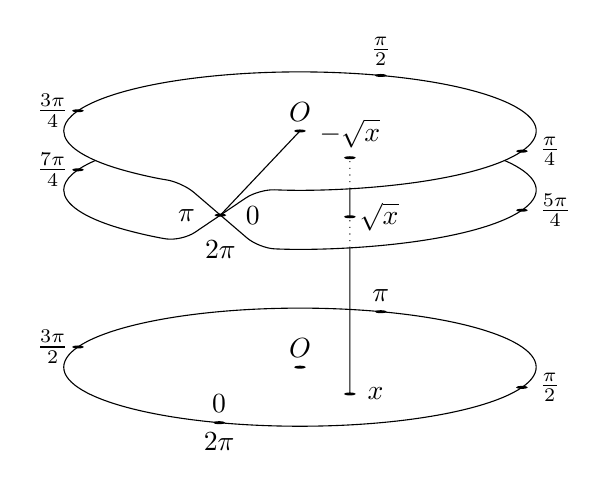
\begin{tikzpicture}[y = {(0,0.25)}, scale=1.5]

	\coordinate (t) at (0,0);
	\coordinate (b) at (0,-2);

	\filldraw[fill=white] ([shift=(-60:2)]b) arc (-60:220:2);
	\filldraw[fill=white] ([shift=(-60:2)]t) arc (-60:220:2);
	\draw[rounded corners=2mm, name path = curve1] ([shift=(220:2)]b) arc
	(220:240:2) -- ([shift=(-100:2)]t) arc (-100:-60:2);
	\draw[rounded corners=2mm, name path = curve2] ([shift=(220:2)]t) arc
	(220:240:2) -- ([shift=(-100:2)]b) arc (-100:-60:2);
	\fill (0,0) circle (0.05) node[above]{$ O $};
	\draw[name intersections={of=curve1 and curve2}] (0,0) -- (intersection-1);
	\fill[name intersections={of=curve1 and curve2}] (intersection-1) circle
	(0.05) node[right=0.2cm]{$ 0 $} node[left=0.2cm]{$ \pi $}
	node[below=0.2cm]{$ 2 \pi $};
	\fill (-20:2) circle (0.05) node[right=0.1cm]{$ \frac{\pi}{4} $};
	\fill (70:2) circle (0.05) node[above]{$ \frac{\pi}{2} $};
	\fill (160:2) circle (0.05) node[left]{$ \frac{3\pi}{4} $};
	\fill ([shift=(-20:2)]b) circle (0.05) node[right=0.1cm]{$ \frac{5\pi}{4} $};
	\fill ([shift=(160:2)]b) circle (0.05) node[left]{$ \frac{7\pi}{4} $};

	\coordinate (-sqrt) at (-65:1);
	\coordinate (sqrt) at ([shift=(-65:1)]b);
	\fill (-sqrt) circle (0.05) node[above]{$ -\sqrt{x} $};
	\fill (sqrt) circle (0.05) node[right]{$ \sqrt{x} $};

	\begin{scope}[yshift = -2cm]
		\draw (0,0) circle (2);
		\fill (0,0) circle (0.05) node[above]{$ O $};
		\coordinate (x) at (-65:1);
		\fill (x) circle (0.05) node[right=0.1cm]{$ x $};
		\fill (-20:2) circle (0.05) node[right=0.1cm]{$ \frac{\pi}{2} $};
		\fill (70:2) circle (0.05) node[above]{$ \pi $};
		\fill (160:2) circle (0.05) node[left]{$ \frac{3\pi}{2} $};
		\fill (250:2) circle (0.05) node[above]{$ 0 $} node[below]{$ 2 \pi $};
	\end{scope}

	\path[name path = function] (x) -- (-sqrt);
	\draw[name intersections={of=function and curve2}] (x) -- (intersection-1);
	\draw[name intersections={of=function and curve2}, dotted] (intersection-1) --
	(sqrt);
	\draw[name intersections={of=function and curve1}] (sqrt) -- (intersection-1);
	\draw[name intersections={of=function and curve1}, dotted] (intersection-1) --
	(-sqrt);

\end{tikzpicture}
\end{document}
